\documentclass[titlepage,11pt,a4paper]{article}
\usepackage[utf8]{inputenc} \usepackage[english]{babel}

% I think these margin options are quite nice
\usepackage[top=1in, bottom=1.25in, left=1.25in,
  right=1.25in]{geometry}

\usepackage{graphicx} \usepackage{float}
\PassOptionsToPackage{hyphens}{url}\usepackage[hidelinks]{hyperref}
\usepackage[titletoc]{appendix}

\hypersetup{ pdfinfo={ Author={SML}, Title={Developer's Guide},
    Creator={LaTeX} } }

\title{Developer's Guide for software from \\Quadcopter ACCESS Summer Project 2015}
\author{Erik Berglund, Paul Rousse, Benjamin
  Summ and Johan Sundin \\at SML, KTH}


\begin{document}
\maketitle \tableofcontents
\newpage

\section{Introduction}
% Short about our project 
This document describes the different parts of the program for
quadcopters developed on the Access Summer Project, 2015, and before,
in the Smart Mobility Lab (SML), KTH.

% The hardware that we used 
The quadcopter type used, and for which this guide is aimed, is the
3DR IRIS$^+$. As a motion capture system Qualisys,
\url{http://www.qualisys.com/}, was used. The quadcopters use the
Pixhawk autopilot. Most parts of the program is written in Python.


\section{Preparations}
This section describes how to set up the different parts of the
program on a fresh computer. Subsec.~\ref{subsec:installation}
describes the installation procedure and
Subsec.~\ref{subsec:configuration} the required configuration
procedure. Finally, some advice are outlined in
Subsec.~\ref{subsec:advice}.

\subsection{Installation}
\label{subsec:installation}
For the main part of the software that was used in the project, the
Linux operating system Ubuntu is recommended, and currently version
14.04 LTS (Trusty). However, some software require a Windows
installation. A short description and the installation procedure for
each required program is found below.

ROS, Robot Operating System, is
a framework aimed at develop software for robots. ROS (currently)
Indigo Igloo can be installed, together with a simulator based on
RotorS, using Gazebo and the PX4 Firmware, using the
instructions at \url{https://pixhawk.org/dev/ros/sitl}. To run the
simulator with several quadcopters, Docker is required. It
can be installed following the instructions at
\url{https://docs.docker.com/installation/ubuntulinux/}.

Scripts and other files from the summer project 2015 can be found at
\url{https://github.com/XXXXXXXXXXXXXXXXXXXX}. It should be cloned
into the \texttt{/src} folder in the ROS workspace. Thereafter, build
the workspace by running \texttt{catkin\textunderscore make} in the
workspace top directory (e.g. in \texttt{/catkin\textunderscore ws}).

To calibrate and change settings of the quadcopters, Mission Planner
can be used. It runs on Windows only. Configuration of the radio can
be done with the 3DR Radio Configuration Tool, also good for checking
the connection strength (RSSI). It is found at
\url{http://ardupilot.com/downloads/?did=89}.


\subsection{Configuration}
\label{subsec:configuration}
Calibrations of the accelerometers of the quadcopters are mandatory
and can be done in Mission Planner. When performing the calibration,
use a water level to setup a flat place. It can be checked that a
calibration was well performed by going to \textit{Flight
 Data}$\rightarrow$\textit{Status}. If $a_x$ and $a_y$ are less than
1\% of $g = 9.8$ and $a_z = -g$ the calibration is satisfactory.

Special conditions apply when flying indoors. Most importantly, the
GPS will stop working. How to disable the GPS and other tips for
flying indoors can be found at \url{http://copter.ardupilot.com/wiki/common-use-cases-and-applications/indoor-flying/}.

For the radio configuration, instructions can be found at
\url{http://copter.ardupilot.com/wiki/common-optional-hardware/common-telemetry-landingpage/common-3dr-radio-version-2/}. Check
that parameters are exactly the same. Also, check that the signal
strength is good (RSSI) with the 3DR Radio Configuration Tool. To
connect the correct antenna to the correct IRIS$^+$ copy
\texttt{/scenarios/launch/99-usb-serial.rules} to the
\texttt{/etc/udev/rules.d/} folder. If only using the antennas in the
SML this is enough (the name of the serial interface of one specific antenna is always
the same). Otherwise, or to add a new antenna, see
\url{http://hintshop.ludvig.co.nz/show/persistent-names-usb-serial-devices/}
or run \texttt{udevadm info -a -n /dev/ttyUSB0 | grep '{serial}' |
  head -n1} and add a line with the result to
\texttt{99-usb-serial.rules}.

\subsection{Advice}
\label{subsec:advice}
There are some general advice when working with IRIS$^+$:

\begin{itemize}
  \item Do not do any modification after an unpacking.
  \item Do not open the IRIS$^+$ if it can be avoided.
\end{itemize}


\section{Architecture}
\label{sec:architecture}

\begin{figure}[h!]                                                               
  \centering \includegraphics[width=\textwidth]{figures/architecture}
  \caption{The architecture used in ROS. Only main parts and
    connections are shown. ``Etc ...'' indicates that other similar
    parts easily can be added. X $= 1, 2, 3, \dots$}
  \label{fig:architecture}                                                              
\end{figure}

The program is using ROS, \textit{The Robot Operating System}, to
connect different parts. A basic knowledge of ROS is
assumed. The architecture used in the program is shown in
Fig.~\ref{fig:architecture}. Circles do not correspond to ROS nodes
strictly, but describe the different parts of the
program. Rectangles, however, correspond to ROS topics. ROS packages
are also written in the figure. Arrows with black head correspond to
publication to a topic, if the arrow points from a circle to a topic,
and subscription to a topic, if the arrow points from a topic to a
circle. Names in the following paragraphs refer to
Fig.~\ref{fig:architecture}.

The goal of the program is to process commands from the user,
forwarded through the GUI, so that the quadcopter, either in the real
world or in the simulator, acts as the user intends. The GUI can start
different ROS launch files, in turn staring scripts that publishes
points for the quadcopter to follow. These scripts are located in the
\texttt{trajectory\textunderscore generator} package, and for example
publishes points for a line or an arc, see
Sec.~\ref{sec:trajectory}. Also, the GUI can publish specific points
itself, not using a predefined script. For more information of the
GUI, see Sec.~\ref{sec:gui}. Apart from commands from the user,
information about the quadcopter's location, speed, acceleration,
pitch, roll and yaw is also needed. This is provided by Qualisys,
taken into the ROS framework by the \texttt{mocap} package.

A controller can be applied, since both the target point and the
current point are known. This is done in the \texttt{controller}
package, see Sec.~\ref{sec:controllers}. The current point is processed by the Security Guard. If not
the quadcopter is within certain safety limits, etc., the Lander
is told to land the quadcopter by the Security Guard. If it is, the
Blender is told to further process the data. For more information
about the Security Guard, see Sec.~\ref{sec:security_guard}. The
blender got it's name because it can ``blend'' outputs of different
controllers and collision avoidance, see Sec.~\ref{sec:blender}. The
outputs of the controllers are then transformed to roll, pitch,
throttle and yaw in the Blender. This is sent to Mavros on the
topic /irisX/mavros/rc/override/ (X $= 1, 2, 3, 4, \dots$) and finally
to the quadcopter.


\section{GUI}
\label{sec:gui}


\section{How to fly}
For experimentation using the GUI two different launch files have to
be started. These are \texttt{mocap.launch} in the \texttt{mocap}
package and \texttt{rqt.launch} in the \texttt{scenarios}
package. Both take an argument called \texttt{simulation}. To start
the mocap one opens a terminal and writes \texttt{roslaunch mocap
  mocap.launch simulation:=false}. To start the GUI one writes
\texttt{roslaunch scenarios rqt.launch simulation:=false}. To connect
to the drone a new terminal is opened by clicking on \textit{New
  Terminal} in the GUI. Then one has to click \textit{Param} and
\textit{Connect}. \textit{Param} has to be clicked in order to load
all the parameters of the drone from the corresponding launch
file. When the connection has been made one can press \textit{Arm} and
the drone should arm. Then different parts of the GUI can be used to
start the drone depending on what one wants to achieve.

\subsection{Advice}
When arming the drone one sometimes gets the error message:
\texttt{Throttle below FS}. This tells you that the throttle is too
low, but usually it is not. One should try to kill the Mavros node,
reconnect and arm again. This almost always does the trick.

If the drone lands because of a problem in the program, the next time
it is armed it might start to go up straight away without having any
controller running. It seems to be possible to avoid this by simply
unplugging the battery and plugging it back in.

If the landing button fails: DO NOT KILL MOCAP. The mechanism to land
via the landing button and mocap is the same and if the landing button
fails it is probable that the whole mechanism has failed. Killing
mocap will only make the drone behave more violently. Instead of
killing mocap disarm the drone manually by holding down the safety
button on the drone. Do not push it again while holding the drone as
it will arm. Shut down and restart all ROS nodes.

Generally, if weird behavior is observed: shut down all the ROS nodes
and restart them to see if the weird behavior stops.

There are some error messages given by Mavros that can be
disregarded. These are DCM bad heading and FCU variance. The DCM bad
heading will make the lamp at the back of the drone blink yellow and
red. This can be disregarded. However, if there is some strange
behavior one should check the status of the drone on Mission Planner.

An unlikely but possible problem is that the combination of markers on
a drone is not unique, i.e. there is another object in the lab that is
confused with the drone by mocap. This is unlikely, but it has
happened.

The performance of the drones seems to be quite sensitive to the
battery level, especially in the z-direction. This has led to a need
of retuning the gravity cancelling constant for different battery
levels. It is rather annoying but necessary. If one manages to get
convergence in the z-direction the integral part stabilizes the drone
in a certain interval of battery levels.

There has been strange behaviour that has remained unexplained. It is
probable that this behaviour emerged from different people messing
with the same code and failing to merge it properly. It is advised to
never work on the same code at the same time as to avoid such
problems.

There has been a need for recalibrating the accelerometers a few
times. It is good to be able to do this calibration rather quickly.

Using the GUI in connection with the launch files enables you to
change the parameters given in the launch file while the drone is in
the air. This is very useful for the tuning of parameters, especially
in connection with the tracking visualizations that are started when
arming the drone. To change the parameters while flying, change them
in the launch file, save it and press \textit{param} in the GUI. If new
parameters are added and you want to use this feature for those
parameters you will have to change the functions that update the
parameters of the blender, PID, obstacle avoidance, etc. If you want
to use this feature for a controller of your own you can add a ROS
service to your controller that calls a function that updates the
parameters. To get this function connected with the GUI you have to
add it in the function called Param() in the script
\texttt{rqt\textunderscore iris.py} in gui/src/gui. As this is used in
the blender and the PID these can be used as examples.

It is advised that somebody operates the GUI at all times in order to
make the drone land in emergency situations.


\section{Trajectory generation and trajectory following}
\label{sec:trajectory}

In the \texttt{trajectory\textunderscore generator} package there are
different scripts that are meant to be used together with a controller
in the \texttt{controller} package (mainly the \texttt{PID}
controller). These scripts generate a reference for the controller
that respects the controller's interface. This means that not only
target positions are generated, but also target velocities and
accelerations. A controller uses these together with the data of the
motion capture system to compute the control output. The interface of
the trajectory generator scripts is defined by the abstract class
called \texttt{Trajectory}. All trajectory generators are subclasses
of this class and use its interface.

There are some classes with class names that end with
\texttt{\textunderscore ext}. These are meant to be used in connection
with controllers that also need a jerk (third derivative of position)
and snap (fourth derivative of position) reference, for example the load
lifting controller (that at the moment of writing unfortunately is not
working).

To calculate the references certain continuous time laws are
used. These depend, of course, on the trajectory to be performed. The
time laws are then discretized using the publishing frequency of the
trajectory node. Each trajectory uses a trajectory node to publish its
data and only one such node should be used within one script. This
assures that the same node is publishing the points all the time and
hence there is no risk of interference between different nodes.

The target points are published on the topic
\texttt{/irisX/trajectory\textunderscore gen/target}, X $= 1, 2, 3,
4, \dots$. The blender subscribes to this topic and passes the
necessary information to the PID.

A useful class in the package \texttt{trajectory\textunderscore
  generator} is the \texttt{TrajectoryGenerator} class. It contains a
collection of different functions that have turned out to be useful
when writing code for trajectory generation. One nice feature is a
function that, given position, velocity and yaw, generates the
corresponding ROS message.

There are also different classes used for leader following. Here,
there also is an abstract base class that can be used for different
ways of leader following.

\subsection{Obstacle avoidance}
\label{subsec:obstacle_avoidance}
In the launch file of each drone there is a parameter called
\texttt{obstacle\textunderscore avoidance}. This parameter can be set to true
or false depending on whether obstacles should be avoided or not. The
obstacles to be avoided are specified through the parameter
\texttt{OBSTACLES\textunderscore TO\textunderscore AVOID}. Observe that an
obstacle that is not registered with the motion capture system or
outside the area of detection will be ignored.

The avoidance itself is done through a potential between the drone and
the obstacle, pushing the drone away from the obstacle. Here the
z-direction is ignored, meaning that the drone is pushed away radially
outward from an infinitely long cylinder whose axis is along the
z-direction in the SML-frame. This is done mainly because two drones
should repel each other even when they are at different
heights. Obviously, it would be of use to improve this algorithm as
one might want the drones to avoid obstacles that are in some finite
interval along the z-axis.


\section{Security guard and lander}
\label{sec:security_guard}

The Security Guard is used for several security features during
experiments. It gives permission to publish on the
\texttt{rc/override} topic either to the Blender, in which case
everything is working satisfactory, or to the Lander, in which case
something went wrong, and the drone lands. Permission is granted to the
lander if:
\begin{itemize}
  \item The motion capture signal is lost for more than 0.5 seconds
  \item The drone is outside the safety zone defined in the launch
    file \texttt{iris\textunderscore nodes.launch}
  \item The landing button in the GUI is pressed
\end{itemize}
Once the landing mode has been initiated it cannot be revoked. That
is, once the Security Guard tells the drone to land it will land. The
system of permissions works through ROS messages containing
booleans. If everything works fine the Security Guard constantly
publishes true on the topic \texttt{irisX/security\textunderscore
  guard/controller} and false on the topic
\texttt{irisX/security\textunderscore guard/lander}. If something goes
wrong the Security Guard publishes false on
\texttt{irisX/security\textunderscore guard/controller} and true on
\texttt{irisX/security\textunderscore guard/lander}. Once the true has
been published on \texttt{irisX/security\textunderscore guard/lander}
there is no chance to take it back. The drone will land. During
landing it is important that the blender does not publish anything on
the texttt{rc/override} topic, otherwise weird behavior can
occur. Therefore, one always has to make sure to publish false at least
once on the topic \texttt{irisX/security\textunderscore guard/controller} to
stop the Blender from publishing. If one uses the Security Guard as it
is implemented this should work without any additions.  

The Lander is a script that sets the landing mode on the APM (the
firmware of the drone) and publishes neutral outputs on the
\texttt{rc/override} topic. This makes the drone land in a controlled
fashion. When the lander works properly the drone goes straight
down. If it does not, i.e. if there is motion in the x- and/or
y-direction, there is something wrong. Probably the controller is
still publishing something on the \texttt{rc/override}. This has to be
fixed, as otherwise the drone behaves unpredictable while landing.


\section{Blender}
\label{sec:blender}

The Blender is found in the \texttt{controller} package. It is used
for two things. The first is taking in acceleration outputs from
different controllers and blending these according to some scheme. The
second is to calculate the control outputs after blending the
accelerations and then publish these on the topic
\texttt{irisX/mavros/rc/override} in order to control the drone.

As of now, the Blender takes an acceleration from a controller and one
from the obstacle avoidance and performs a convex combination of
these. The constant with which the acceleration from the obstacle
avoidance is weighted is dependent on the distance to the
obstacle. The Blender uses a method of the obstacle avoidance to get
this constant. Of course, if obstacle avoidance is turned off the
output is only calculated from the output of the controller.

Currently, there is a problem with this kind of blending of
accelerations. The problem is that convergence to a goal point cannot
be guaranteed in this way. In fact it can be easily thought of an
example where convergence does not occur. Assume that the quadcopter
is hovering at a certain point, which is its target, and another
quadcopter is approaching. Furthermore, assume that the first
quadcopter tries to avoid the second one, but the second one does not
try to avoid the first. Then the first one will move away from its
target and hover at a different point. Thus it is clear that a more
sophisticated controller is necessary in order to do precision based
tasks involving collision/obstacle avoidance.


\section{Controllers}
\label{sec:controllers}
Mainly the PID controller, Sec.~\ref{subsec:pid}, has been used in
this project. However, a new controller can easily be added by
modifying the Blender, Sec.~\ref{sec:blender}, and using the interface
provided by the abstract base class \texttt{Controller}.

\subsection{PID controller}
\label{subsec:pid}
The PID controller in the \texttt{controller} package is not just a
normal PID controller. The proportional and derivative gains are
coupled in a certain way. It is therefore not possible to change these
gains independently by using the parameters given in the launch
files. If they have to be changed independently one can either change
them directly in the script of the PID without using the coupling
between them or one can change the damping constant named
\texttt{x\textunderscore i} in the script of the controller. It has
not really been necessary to do this, however.  It should be
sufficient to change the parameters \texttt{CONTROL\textunderscore
  CANCEL\textunderscore GRAVITY}, \texttt{PID\textunderscore w},
\texttt{PID\textunderscore w\textunderscore z},
\texttt{PID\textunderscore I\textunderscore lim},
\texttt{PID\textunderscore} \texttt{K\textunderscore i},
\texttt{PID\textunderscore I\textunderscore lim\textunderscore z} and
\texttt{PID\textunderscore K\textunderscore i\textunderscore z}. The
first parameter is crucial for performance in the z-direction as it is
used to counterbalance gravity. It has been observed that this
parameter might have to be retuned for different battery levels. The
next two parameters are used to adjust both the proportional and the
derivative gain in an optimal way with respect to each other. The
\texttt{PID\textunderscore w} is for x and y and
\texttt{PID\textunderscore w\textunderscore} z is for z. The
\texttt{I\textunderscore lim} and \texttt{K\textunderscore i} are the
saturation and gain of the integral term. The ones with
\texttt{\textunderscore z} in the end are for the z-direction, the
other ones for x and y. There is no need for a high saturation limit
in the x and y direction but in the z direction it should be rather
high to guarantee robustness against the change in battery level. The
parameters that currently are in the launch files work fine for iris2,
iris3 and iris4.  Observe that the value of the parameters
\texttt{Kphi} and \texttt{Ktt} should be 637 for both.


\section{Connecting servos}
\label{sec:servos}
IRIS$^+$ uses the Pixhawk autopilot. On the Pixhawk there are outputs
for servos, shown in Fig.~\ref{fig:pixhawk_outputs}. The outputs are
divided in eight ``main outputs'', MAIN OUT 1-8, and six ``auxiliary
outputs'', AUX OUT 1-6. MAIN OUT 1-4 are occupied by the the four
motors. However, MAIN OUT 1-8 should be avoided for servos anyway
since these update at a rate of 400 Hz by default. AUX OUT 1-6 update
at 50 Hz -- standard for servos.

\begin{figure}[h!]                                                               
  \centering
  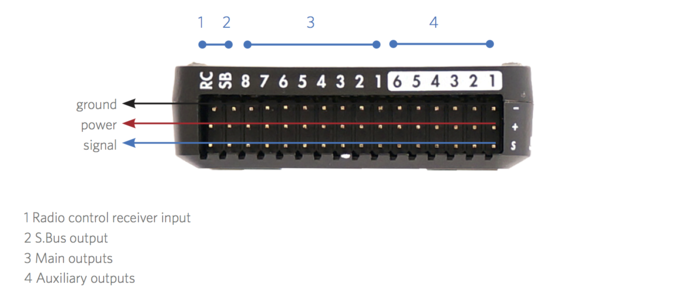
\includegraphics[width=1.0\textwidth]{figures/pixhawk_outputs}
  \caption{Pixhawk outputs for servos. Image from
    \url{http://copter.ardupilot.com/wiki/common-autopilots/common-pixhawk-overview/}.}
  \label{fig:pixhawk_outputs}                                                              
\end{figure}

AUX OUT 5-6 are, by default, set up as relays. The number of AUX OUT
ports set up as servo outputs can be changed in Mission Planner with
the \texttt{BRD\textunderscore PWM\textunderscore COUNT} parameter, in
the way that setting \texttt{BRD\textunderscore PWM\textunderscore
 COUNT} to 6 gives servo output on AUX OUT 1-6.

The IRIS$^+$ transmitter and receiver has eight channels. This is
reflected in the way that a vector of eight components can be sent to
the quad via the topic \texttt{/irisX/mavros/rc/override/}. The first four
components are for roll, pitch, throttle and yaw, leaving the other
four for servos. In addition to that, the different channels need to
be linked to the different servo outputs on the Pixhawk. This can
be done in the Mission Planner. In Mission Planner, the eight channels
are named RC1-RC8. The different servo ports are named in a similar
way: RC1-RC8 corresponds to MAIN OUT 1-8 and RC9-RC14 corresponds to
AUX OUT 1-6. Unfortunately, in the current version of Mission Planner,
there is no general way of connecting channel RCX to RCY, X $= 1 \dots
8$, Y = $= 1 \dots 14$. If three or less servos are needed, the built
in settings for a camera gimbal can be used.\footnote{Which signals to
be sent to which servo output are controlled by the parameter
\texttt{RCX\textunderscore FUNCTION}, X $= 1 \dots 14$, in Mission
Planner. For these parameters, there is an option called
\texttt{Passthrough}, passing channel X to output X, but since there
are eight channels, only MAIN OUT 1-8 can be reached by this option,
not AUX OUT 1-6.}

The Pixhawk does not provide power to the servos itself, so these must
be powered in other ways. A BEC or ESC, providing 5 V, can be used,
for example. It can be connected to the servo outputs on the Pixhawk
or to a servo directly. By default, the ground pins are connected to
the ground of the battery, by a wire to MAIN OUT 1 ground pin. Also,
on the bottom of the IRIS$^+$ there are a black cable connected to AUX
OUT 6 ground pin and a white cable connected to AUX OUT 1 signal
pin. In addition to this, there is a red power cable and another black
ground wire connected to the battery of the IRIS$^+$, providing 12
V. If the voltage is lowered to around 5 V this can be used. So, if
only one servo is needed, the quadcopter does not even needs to be
opened!

For additional tips and tricks, see
\url{http://copter.ardupilot.com/wiki/common-optional-hardware/common-servo/}
and \url{https://learn.adafruit.com/quadcopter-spray-can-mod/}. A
wiring diagram for the Pixhawk can be found in
\url{http://copter.ardupilot.com/wiki/advanced-pixhawk-quadcopter-wiring-chart/}.


\newpage
\begin{appendices}
\begin{center}
  {\bf APPENDIX}
\end{center}

\section{``Fix my IRIS'' procedure}
If the IRIS$^+$ starts to behave strange, a standard procedure is
outlined below, fixing many of the possible errors.

\begin{itemize}
  \item Put a fully charged battery in the drone.
  \item Is the drone unstable? In that case, try to control it with the RC
    transmitter.
    \begin{itemize} 
      \item In case of good behavior, check the controller.
        \begin{itemize}
          \item Is hovering term too high?
          \item Is the gains too high?
        \end{itemize}
      \item If drone fails to arm, take a look at messages in Mission
        Planner.
      \item If propellers have different speeds, do a ESC Calibration.
      \item If not stable with RC transmitter:
        \begin{itemize}
          \item Redo accelerometer calibration.
          \item Redo compass calibration.
        \end{itemize}
      \item If the range of the RC transceiver is low:
        \begin{itemize}
          \item Redo RC transmitter calibration.
          \item Change the battery of the drone.
          \item Change the RC transmitter batteries.
        \end{itemize}
    \end{itemize}
    Otherwise, redo calibration in Mission Planner and be careful that
    there is no offset in the RC command (neutral position must be
    equal to 1500).
  \item Does Mavros fail to connect?
    \begin{itemize}
      \item In case of green light blinking, check 3DR radio
        configuration.
      \item Check USB connection.
      \item Check configuration of the launching file (e.g. \texttt{iris1.launch}).
      \item Don't get parameters?
        \begin{itemize}
          \item Reboot Mavros or reboot the drone.
          \item Lower the air speed parameter of the 3DR radio.
          \item As an alternative, take the time and wait for all the
            parameters.
        \end{itemize}
      \item In Mission Planner, check compass health and read
        \url{http://ardupilot.com/forum/viewtopic.php?f=48&t=10478}
        (don't move the quad and don't close the battery slot during gyro
        initialisation).
    \end{itemize}
  \item ULTIMATE FIX: Change the drone! (Drones are complex systems -- it
    might be difficult to find the error.)
\end{itemize}
    
\section{3DR Radio communication interference}
It seems that the radios interfere when they are close, so try to have
at least 1 meter between each of them.  However, it is not sufficient,
if you look at the /diagnostics topic, then you will see that there
are many Rx errors, it is the same in Mission Planner, by looking at
the logs, we see that many errors append. One of the consequence that
is directly visible is that that parameters are much slower to be
loaded at the initialisation of Mavros.

A quick fix as been made by just decreasing the timeout variable in
the \texttt{mavros} package (file in
\texttt{mavros/src/plugins/param.cpp}, \texttt{PARAM\textunderscore
  TIMEOUT\textunderscore MS} has been changed to 100 ms instead of
1000 ms and \texttt{RETRIES\textunderscore COUNT} has been increased
to 5). In this way the initialisation is faster, however it does not
solve this Rx trouble, and it might have some consequences on the
controller if too many errors happens.  Try to reduce the numbers of
data that are transmitted by using the "rosrun mavros mavsys rate"
command.

A good fix will be to find a firmware were the ECC can correct more
that 25\% of errors through the communication protocol. However, it is
not possible without getting inside the firmware code. I (Paul) did
not managed to make the "LBT Rssi" work (listen before talk); it could
help to reduce the number of Rx errors. A good parameter to tune is
the Protocol, setting up to Raw Data might increase the rate at which
we can transmit data through \texttt{rc/override}. However, as long as
I am not sure that every thing work well, I will leave it on Mavlink.
The Tx power does not have to be extremely high, the 3DR radio is made
so that it can transmit data up to 500 m, since we are about 10 m of
the quad, it is okay to set it to 5.

Some people have been facing similar problems. However, none of the
fix worked (trying with the 1.7 firmware for the 3DR radio, setting
different \texttt{SYSID\textunderscore THISMAV}, separate every
frequencies for each coupled radios). Some links are
\\ \url{http://copter.ardupilot.com/wiki/common-optional-hardware/common-telemetry-landingpage/common-3dr-radio-version-2/}
\\ \url{http://ardupilot.com/forum/viewtopic.php?f=22&t=8488}
\\ \url{http://www.rcgroups.com/forums/showthread.php?t=2077354}
\\ \url{http://ardupilot.com/forum/viewtopic.php?t=10000&p=24499}
\\ \url{http://diydrones.com/forum/topics/question-on-using-multiple-3dr-radios-to-control-multiple-drones}

Documentation can be found at
\url{http://copter.ardupilot.com/wiki/common-optional-hardware/common-telemetry-landingpage/common-3dr-radio-advanced-configuration-and-technical-information/#Upgrading-radio-firmware}

To get any version of the Firmware, clone
\url{https://github.com/Dronecode/SiK} and get back to another commit
(the one of the version you want), install sdcc with \texttt{apt-get},
do a \texttt{make install} in the Firmware directory, the hex file
(equal to the firmware) is the \texttt{Firmware/obj/hm\textunderscore
  trp/radio$\sim$hm\textunderscore trp/radio$\sim$hm\textunderscore trp.ihx}.

\end{appendices}

\end{document}
